\documentclass{article}
\usepackage{tikz}
\begin{document}

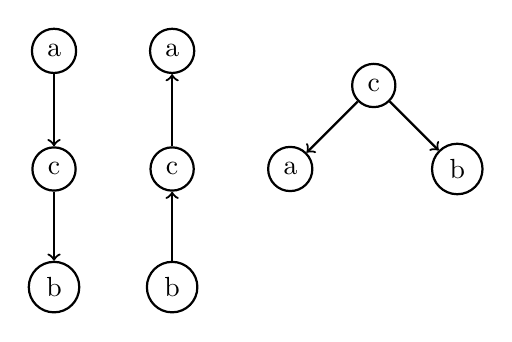
\begin{tikzpicture}[node distance={15mm}, thick, main/.style = {draw, circle}]
    \node[main] (a) {a};
    \node[main] (c) [below of=a] {c};
    \node[main] (b) [below of=c] {b};

    \node[main] (d) [right of=a] {a};
    \node[main] (e) [below of=d] {c};
    \node[main] (f) [below of=e] {b};

    \node[main] (g) [right of=e] {a};
    \node[main] (h) [above right of=g] {c};
    \node[main] (i) [below right of=h] {b};

    \draw[->] (a) -- (c);
    \draw[->] (c) -- (b);

    \draw[->] (f) -- (e);
    \draw[->] (e) -- (d);

    \draw[->] (h) -- (g);
    \draw[->] (h) -- (i);

\end{tikzpicture}
\end{document}
